\documentclass{article}
\usepackage{amsmath}
\usepackage{hyperref}
\usepackage{graphicx}
\begin{document}
\begin{titlepage}
\title{EE 239AS \\Special Topics in Signals and Systems\\Project 2\\Classification Analysis\\Winter 2016} 
\author{Liqiang YU, Kaiming WANG and Jun FENG\\
904592975, 504592374, 304588434} 
\date{02-21-2016}
\end{titlepage}

\maketitle
\newpage
\tableofcontents
\newpage
\section{Introduction}
In this report, we implemented some classification models to classify the textual data from the "20 Newsgroups" dataset, including support vector machine (SVM), naive Bayes classifier and logistic regression classifier. Before the classification,there were some data preprocessing steps, like changing the number in each subset to make them balanced, transforming the textual data into TF-IDF matrix, implementing the singular value decomposition to reduce the dimension of TF-IDF matrix. The task included binary classification and multiclass classification. The results were measured with the metrics including the average of precision, recall and accuracy. Moreover, in order to characterize the trade-off between true positive rate (TPR) and false positive rate (FPR), the receiver operating characteristic (ROC) curve was plotted.\\
\\
The report is organized as follows: in section \ref{sec:binary} we discussed the classification results with support vector machine, naive Bayes classifier and logistics regression classifier. We compared the results from two SVM models : hard margin SVM and soft margin SVM, computed the precision, recall, accuracy and confusion matrix, plotted the ROC curve from three models. In section \ref{sec:multi}, we implemented two strategies for multiclass classification : "one VS one" and "one VS rest" and repeated the above procedures to test the results.
\section{Binary Classification}\label{sec:binary}
In the binary classification problem, we chose eight classes and wanted to seperate them into two classes : Computer Technology and Recreational Activity. We assign the tag 0 to Computer Technology subclasses and tag 1 to Recreational Activity subclasses. The number of each subclass is almost the same so there is no need to balance them.
\subsection{Hard Margin SVM}
In the hard margin SVM, the objective function is
\begin{equation*}
min \frac{1}{2}\Vert W \Vert _2 ^2
\end{equation*}
And the constraints is
\begin{equation*}
y_i(W^T\overrightarrow{x_i}+b)\geq 1, i\in\lbrace 1, ..., n \rbrace
\end{equation*}
\\
In the program, we set C to 100000 to simulate the effect of hard margin. The average precision is 96.61\%, the average recall is 98.49\% and the accuracy is 97.49\%.The confusion table is shown in Table \ref{tb:confu}. The ROC curve  is shown in figure \ref{fig:roc}
\begin{table}
\begin{center}
\caption{The confusion matrix of hard margin SVM}
\label{tb:confu}
\begin{tabular}{|c|c|c|}
\hline
& Predicted Comp& Predicted Rect\\
\hline
Actual Comp&1505&55\\
\hline
Actual Rect&24&1566\\
\hline 	
\end{tabular}
\end{center}
\end{table}

\begin{figure}[htbp]
\centering
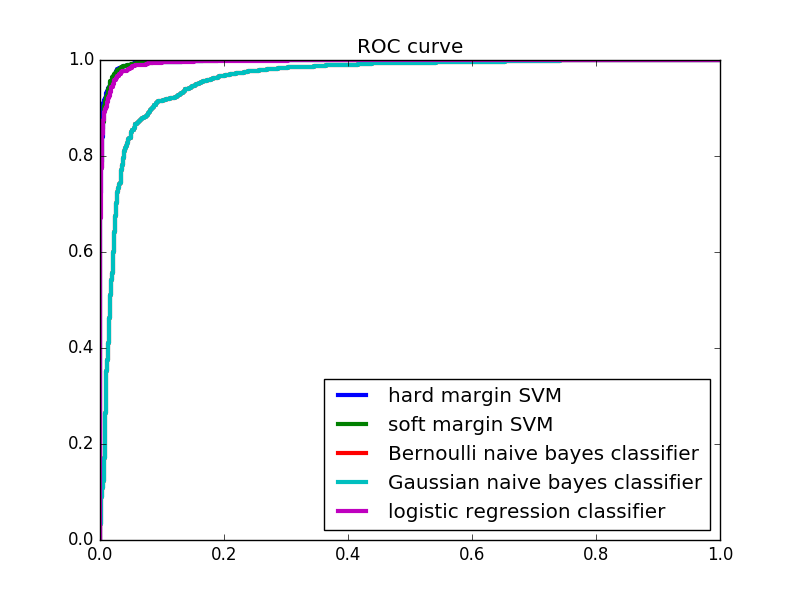
\includegraphics[width=.6\textwidth]{roc.png}
\caption{The ROC curve of hard margin SVM}
\label{fig:roc}
\end{figure}
\subsection{Soft Margin SVM}
The problem of the hard margin model is that it may overfit the data, therefore it's better to use the soft margin SVM. In the soft margin model, we add error parameter in the objective function and the constraints. Thus the objective function is changed to the following:
\begin{equation*}
min \frac{1}{2}\Vert W \Vert _2 ^2 + \gamma\sum_{i=1}^{n}\xi _i
\end{equation*}
\\
Accordingly, the constraints are changed to the following:
\begin{equation*}
y_i(W^T\overrightarrow{x_i}+b)\geq 1-\xi _i,  \xi _i \geq0,  i\in\lbrace 1, ..., n \rbrace
\end{equation*}
\\
The $\gamma$ is the hyperparameter here and different $\gamma$ will affect the classification results. We implemented 5-fold cross validation to fit the model and choose the $\gamma$.  The best $\gamma$ we can get is 1000. The average precision is 96.61\%, the average recall is 97.96\% and the accuracy is 97.27\%. The confusion matrix is shown in Table \ref{tb:confu_soft}
\begin{table}
\begin{center}
\caption{The confusion matrix of soft margin SVM with $\gamma$ = 100000}
\label{tb:confu_soft}
\begin{tabular}{|c|c|c|}
\hline
& Predicted Comp& Predicted Rect\\
\hline
Actual Comp&764&27\\
\hline
Actual Rect&16&769\\
\hline 	
\end{tabular}
\end{center}
\end{table}
\section{Multiclass Classification}\label{sec:multi}
\section{Conclusion}
In this project, we aimed to finish some classification tasks with the textual data provided by the "20 Newsgroup" dataset. We classified 8 subclasses into 2 classes with the hard margin SVM, soft margin SVM, naive Bayes classifier and logistics regression classifier. The comprehensive results is shown in the Table \ref{tb:binaryresults}. As for the multiclass classification, the comprehensive results is shown in Table \ref{tb:multiresults}.
\begin{table}
\begin{center}
\caption{The comprehensive results of binary classification}
\label{tb:binaryresults}
\begin{tabular}{|c|c|c|c|}
\hline
& Accuracy& Precision& Recall\\
\hline
hard margin SVM& 97.49\%&96.61\% &98.49\% \\
\hline
soft margin SVM& 97.27\%&96.61\% &97.96\% \\
\hline 	
Bayes& & & \\
\hline
Logistic Regression& & &\\
\hline
\end{tabular}
\end{center}
\end{table}

\begin{table}
\begin{center}
\caption{The comprehensive results of multiclass classification}
\label{tb:multiresults}
\begin{tabular}{|c|c|c|c|}
\hline
& Accuracy& Precision& Recall\\
\hline
SVM& \%&\% &\% \\
\hline
Bayes& & & \\
\hline
Logistic Regression& & &\\
\hline
\end{tabular}
\end{center}
\end{table}
\end{document}